\documentclass[]{article}

% math packages
\usepackage{amsmath}
\usepackage{amsthm}
\usepackage{bm}

% for coloring in a table
%\usepackage[table,xcdraw]{xcolor}

% including graphics
\usepackage{graphicx}
\graphicspath{ {./images/} }

% drawing graphs
\usepackage{tikz-cd}
\usepackage{tikz}
\usetikzlibrary{shapes.geometric, arrows}
\tikzstyle{startstop} = [rectangle, rounded corners, minimum width=3cm, minimum height=1cm,text centered, draw=black, fill=red!10]
\tikzstyle{arrow} = [thick,->,>=stealth]

% hyperlinks
\usepackage{hyperref}

% some useful shortcuts
\DeclareMathOperator*{\argmax}{argmax}
\newcommand{\indep}{\perp\!\!\!\!\perp}
\newcommand{\blambda}{{\bm{\lambda}}}
\newcommand{\btheta}{{\bm{\theta}}}
\newcommand{\bpsi}{{\bm{\psi}}}

\newcommand{\by}{\mathbf{y}}

\usepackage{setspace}
\doublespacing

% Editing macros
\usepackage{color}
\newcommand\cmnt[2]{\qquad{{\color{red} \em #1---#2} \qquad}}
\newcommand\cmntM[1]{\cmnt{#1}{Miratrix}}
\newcommand\cmntC[1]{\cmnt{#1}{Che}}
\newcommand\awk{{{\color{red} {$\leftarrow$ Awkward phrasing}}\qquad}}
\newcommand\cmntMp[1]{{\color{red} $\leftarrow$ {\em #1 -Miratrix} \qquad}}



%opening
\title{Power calculations for detecting \\ individual site impacts}
\author{Jonathan Che \& Luke Miratrix}

\begin{document}

\maketitle

%\begin{abstract}
%\end{abstract}


\section{Introduction}

The usual question for multisite trials\textemdash randomized trials where each of a set of sites has individuals randomized into treatment and control\textemdash is whether the treatment worked \emph{on average overall}, even though the treatment may have different effects across sites.\footnote{Though seemingly simple, even this question has its wrinkles if we believe the site-level average effects differ.
For example, do we estimate the average impact for all individuals across all sites, or instead estimate the simple site average of their average impacts?}
When designing a multisite experiment there are power analysis tools designed to ensure a given design will achieve desired levels of power for this average effect.
There are even power formulas designed to ensure one can detect a given level of cross-site impact variation, if that is a quantity of interest.

But what if we are interested in the individual sites?
Typically, in a multisite experiment no individual site will be large enough to be well-powered, on its own, for detecting whether treatment at that site was actually effective.
This is, after all, why we frequently turn to multisite experiments: we seek to increase our overall power by averaging across a collection of underpowered, local, investigations.
That being said, the stakeholders at these local investigations will frequently want to know not whether the experiment worked overall, but whether it worked for them.
As researchers, we might also want to identify which sites are most likely to be the drivers of an overall effect.

We can get an approximate answer to these questions about individual sites by using multilevel or hierarchical Bayesian models to partially pool the individual site effects.
For each site, these models ``borrow strength'' from the other sites under the assumption that the sites are related.
This process results in point estimates for each of the individual sites that are shrunken towards the overall average estimated effect.

The construction of confidence intervals around these shrunken estimates requires some nuance.
In general, confidence intervals for individual site effects in a hierarchical model are ill-defined under a frequentist framework.\footnote{Under a frequentist framework, the individual site effects $\tau_j$ are random effects, and not parameters of interest.
Just as it makes little sense to define confidence intervals for regression residuals, it makes little sense to define confidence intervals for these random effects.
(To be honest, I'm not positive about this intuition.
Section 1.2 of  \href{https://core.ac.uk/download/pdf/38903061.pdf}{this paper} describes frequentist inference for random effects, though it mentions that it's quite messy.
On the other hand, the internet (e.g., \href{https://stat.ethz.ch/pipermail/r-sig-mixed-models/2011q3/014077.html}{here} or \href{https://github.com/lme4/lme4/issues/497}{here}) suggests that people don't really do frequentist inference on the random effects.) }
We can, however, construct credible intervals under a Bayesian framework that can provide similar information about the uncertainty in site effects.
There is an extensive literature concerning the construction of appropriate intervals for individual site effects under shrinkage (see Casella and Hwang (2012) for a thorough review; see He (1992), Hwang et al. (2009), and Armstrong et al. (2021) for relevant examples of these methods).

Unfortunately, these credible intervals do not satisfy the frequentist definition of $\alpha$-level converage for the $\tau_j$ values; instead, they satisfy so-called Empirical Bayes (EB) coverage, which integrates the coverage probability over both the data and the parameters (Morris 1983).\footnote{Recall that frequentist coverage is defined as the probability that a random interval contains a fixed parameter $\theta$, where randomness is integrated over the distribution of the observed data.
	EB coverage additionally integrates out the parameter $\theta$ over its prior distribution.}
This means that they only provide guarantees for \textit{average} coverage across sites, and not for coverage for any particular site.
These guarantees are not sufficient for stakeholders in multisite trials who are specifically interested in knowing whether the experiment worked for their site.
For example, the inherent bias in shrunken point estimates raises concerns that only examining average coverage could mask systematic undercoverage for sites with extreme effects, which would be a problem for stakeholders at such sites.
Overall, the question of inference for particular site effects in multilevel models appears to remain fairly open (Armstrong et al (2021) cites Hansen (2006) for this), with limited guidance about best practices.

In this study, we focus on frequentist-style conditional power analyses for detecting a hypothesized effect for a specific site in a particular study design.\footnote{I.e., we are interested in power/coverage conditional on given $\tau_j$ values, and not in average power/coverage across the collection of $\tau_j$ values in a multisite trial.}
While there is an extensive literature on these types of power analyses for the overall average treatment effect and cross-site variation in multisite trials (e.g., Raudenbush \& Liu 2000, many others...), less attention has been paid to similar power analyses for individual site effect estimates.
We first review how one might use multilevel and Bayesian models to report such effects.
We then propose simulation-based tools to do power calculations.
Finally, we conduct a simulation study to examine power for site-level treatment effects in multisite trials.
At this point, we also examine how poorly these site-level estimates perform in practice, and provide guidance on the overall business of individual site-effect estimation in the context of multisite trials.


\section{Detecting individual site effects}

Assume a Normal multilevel model for individuals $i$ in sites $j$ of: 
\begin{align*}
	Y_{ij} &= \alpha_j + \tau_j Z_{ij} + \epsilon_{ij} \\
	\alpha_j &= \alpha + u_{0j} \\
	\tau_j &= \tau + u_{1j} \\
	\begin{pmatrix}
		u_{0j} \\ u_{1j}
	\end{pmatrix} &\sim N\left(
	\begin{pmatrix}
		0 \\ 0
	\end{pmatrix}, 
	\begin{bmatrix}
		\sigma^2_\alpha & \rho_{01} \\ \rho_{10} & \sigma^2_\tau
	\end{bmatrix}\right) \\
	\epsilon_{ij} &\sim N(0, \sigma^2_y) ,
\end{align*}
for individual outcomes $Y_{ij}$, individual treatment indicators $Z_{ij}$, random site intercepts $\alpha_j$, and random site treatment effects $\tau_j$.

We simulate data under this model, using some simplifying assumptions.
We set $\rho_{10} = \rho_{01} = 0$ so that intercept and treatment random effects are uncorrelated.
We also fix $Var(Y_{ij}(0)) = Var(\alpha_j) + Var(\epsilon_{ij}) = 1$ so that the control-unit outcomes are in effect size units.
This scaling gives the variance of our random intercepts in terms of the Intra Class Correlation Coefficient (ICC) of:
$$ICC = \frac{Var(\alpha_i)}{Var(\alpha_j) + Var(\epsilon_{ij})} = Var(\alpha_j) = \sigma^2_\alpha$$
This also dictates that the within-site residual variation must be $\sigma^2_y = 1-ICC$ so that the control-unit outcomes have variance 1 within each site.
We ignore additional covariate adjustments for the moment for clarity.

The simplest, completely unpooled test of whether there is a positive treatment effect within site $j$ would be to drop the rest of the data and test the difference in means of the treatment and control groups within site $j$.
The power to detect effects locally in this manner is purely a function of the site sample size, variation in outcomes within the site, and the size of the true site average impact.
The typical formula for the standard error for site $j$'s impact estimate would then be:
$$ SE_j = \left[ \frac{1}{n_j} \frac{1}{(1-p_j)p_j} (1-ICC) \right]^{1/2} , $$ 
where $p_j$ is the proportion treated at site $j$.
For testing, we would estimate $\hat{\tau}_j$ and $\widehat{SE}_j$, the latter with a plug-in estimate of $\hat{\sigma}_j$.\footnote{For two examples, we could estimate $\hat{\sigma}_j$ with an interacted linear regression where we completely pool our residual variation across sites, or simply estimate the within-group variation at site $j$.
The former would help stabilize, under homoscedasticity, our residual estimate which could be helpful in very small sample contexts.}
We would finally obtain $p$-values using $t = \hat{\tau}_j / \widehat{SE}_j$, referenced to a $t$ distribution with many degrees of freedom, assuming the site is not tiny.

A multisite analysis pools data across sites to try to improve effect estimates.
With a multilevel model, we first estimate the overall parameters, including the degree of cross site variation $\omega$, and none of the individual site average impacts.
We then, in a second step, effectively shrink all the raw $\hat{\tau}_j$ towards the overall estimate of $\hat{\tau}$ to get $\tilde{\tau}_j$, shrinking more the lower our estimate of $\omega$ is.
These $\tilde{\tau}_j$ are the Empirical Bayes estimates for the individual site impacts; while biased, they are known to be better point estimates (in terms of mean-squared error) for the full collection of true site-level impacts than the raw estimates $\hat{\tau}_j$ (cite something here).

Under a parametric or empirical Bayes framework, we can also obtain standard error estimates $\tilde{SE}_j$ for our $\tilde{\tau}_j$.
Using the estimate and standard error, we can finally conduct hypothesis testing as before, taking the test statistic of $t = \tilde{\tau}_j / \tilde{SE}_j$ as standard normal statistic and calculating a $p$-value as usual.
As discussed in the introduction, however, confidence intervals constructed using these standard errors do not satisfy frequentist coverage criteria, where, e.g., for a fixed $\tau_j$ the interval $(\tilde{\tau}_j \mp 1.96 \tilde{SE}_j)$ would cover $\tau_j$ 95\% of the time over repeated samples of the data.
Instead, they satisfy EB coverage, where appropriate coverage holds over repeated samples of the data \textit{and} $\tau_j$ from the data-generating Normal model.
In other words, hypothesis tests run in this way will not have the usual guarantees on Type-I error rate control for the site-specific effects.
That being said, they may perform decently well in practice.

Without shrinkage, power is simply a function of the un-shrunk standard error $SE_j$ and the true average effect $\tau_j$ for site $j$.
Given the shrinkage, the power to detect an individual site effect will additionally depend on the general size and distribution of average effects at other sites.
Of course, the most relevant parameter will be the site's average effect, but the distribution of impacts estimated at the other sites will affect how each site estimate is shrunk towards the overall average impact.
The question is how much this shrinkage helps or hurts the power and validity of the testing procedure, especially for those sites that actually have impacts far from the overall average.


\section{A simulation-based power calculator}

To calculate power for a multisite trial, we need to specify parameters for both the individual site of interest and its context.
While a typical power analysis for a single site only requires specification of a single hypothesized effect size (along with significance and power requirements), in a multisite trial the site's context, i.e., the number, size, and distribution of other sites, will also affect the effect estimate for that site.
The question is then: for a given site of interest, within a given context of interest, what is the chance of rejecting the null of no effect for that site?

We answer this question via simulation.
We repeatedly generate our target site and an associated context, analyze the synthetic data, and record whether we have detected an effect.
The frequency with which we reject the null across our simulations is then the power for that site and context.
We propose three general tools for conducting such a simulation.

\paragraph{Set-site simulation.} A straightforward way to conduct a multisite power simulation is to specify the site, and then to separately specify the sites in its context.
This completely decouples the site from its context.
For example, we could set the value of the true effect for site 1 to be $\tau_1 = 7$, and then sample the true effects for the $J-1$ other sites as $\tau_2, \dots, \tau_J \sim N(\tau, \omega)$.
For each set value of $\tau_1$, we could repeatedly generate data from a context to determine the power for that site/context combination.

This simulation strategy has two unusual features.
First, the full collection of sites 1 through $J$ no longer matches any data-generating model, because the site of interest is manually specified, unlike its context, which is still randomly generated according to particular parameters.
Second, for a fixed context, changing the site effect of interest naturally changes features of the full dataset on which the model is fit.
For example, if we fix the context as $\tau_2, \dots, \tau_J \sim N(\tau, \omega)$, setting $\tau_1 = -10$ versus $\tau_1 = 10$ will change $\bar{\tau} = \frac{1}{J} \sum_{j=1}^{J} \tau_j$, so even though the context remains the same, the direction in which the model shrinks its effect estimates can change.
We therefore need to be careful when interpreting comparisons across different $\tau_0$ values given a particular context.
That being said, the set site approach provides a clean answer to the question: if my site of interest is as specified, and it is otherwise within a particular context, what is the chance that I detect an effect for it?

\paragraph{Remove-site simulation.} Another way to conduct a multisite power simulation is to first specify and simulate all $J$ sites, and to then choose a particular site as the ``site of interest'' and remove it from its ``context,'' which would consist of the remaining $J-1$ sites.
This can be done for each of the generated sites in every simulation.
If we repeatedly do this, we can get power curves by grouping together sites that happen to have the same true impacts and seeing how often we reject the null for them.\footnote{Of course, given the continuous nature of the random site effects $\tau_j$, sites will never have the exact same true effect.
	We therefore round the randomly generated $\tau_j$ to the nearest 0.05 before generating the individual responses within sites.
	Alternatively, we could, e.g., repeatedly simulate data from a context where $\tau_j \sim N(0, 1)$, and summarize the power for all sites for which the true $\tau_j \in [0.95, 1.05]$ to estimate  power for sites with $\tau_j$ ``near'' 1, repeating this for $\tau_j$ values ``near'' as many other values as we'd like.}

This approach, however, has an undesirable feature.
Suppose we want to know the power for a site with $\tau_j = 1$ in the context $N(\tau, \omega)$.
When computing this power, we would systematically exclude all sites with $\tau_j = 1$ from the context; in other words, our true context would be $N(\tau, \omega \mid \tau_j \neq 1)$, the usual context with a gap at the specified $\tau_j$ value.
Besides making things difficult to interpret, this phenomenon also makes it hard to compare results across different $\tau_j$ values, since the context always changes.
As such, we opt to not employ this simulation strategy.

\paragraph{All-site simulation} One final way to conduct a multisite power simulation is to use remove-site simulation, but to treat the full collection of $J$ sites as the ``context'' for each site of interest instead of only considering the $J-1$ other sites as the context.
This approach circumvents the previous complications regarding the data-generating distribution; data are generated exactly according to the theoretical model, and there are no gaps or additions caused by removing or adding $\tau_j$ values for the site of interest.

All-site simulation, however, still runs into similar complications as set-site simulation.
Because each site of interest is included within its ``context,'' sites of interest with higher $\tau_j$ values will naturally have contexts with higher $\bar{\tau}$ values, on average.
As with set-site simulation, we need to be careful when interpreting comparisons across $\tau_j$ values for a fixed context.
%For a given context $G(\cdot)$, there is natural variation between simulations of $\tau_1, \dots, \tau_J \sim G(\cdot)$; in particular, some simulations will have higher true $\bar{\tau} = \frac{1}{J} \sum_{j=1}^J \tau_j$ values and others will have lower $\bar{\tau}$ values, simply due to random chance, especially if $J$ is small.
%When we summarize the results for higher values of $\tau_j$ across simulation runs of the same theoretical context $G(\cdot)$, we notice that those higher-$\tau_j$-value sites come from simulated contexts with higher $\bar{\tau}$ values, on average.
%In other words, because we include the sites of interest within their ``contexts,'' sites of interest with higher $\tau_j$ values will naturally have contexts with higher $\bar{\tau}$ values.
%Given a fixed context-generating distribution $G(\cdot)$, this makes comparison across different $\tau_j$ values for the site of interest quite challenging, because the higher $\tau_j$ values come from simulations with higher $\bar{\tau}$ values.
Another minor challenge with the all-site approach is that we cannot directly specify the $\tau_j$ values of our sites of interest, which means that the range of possible $\tau_j$ values (and how frequently extreme $\tau_j$ values appear) is constrained by our context.

As a result, all-site simulation answers a slightly different question than does set-site simulation: if I have a particular context and am interested in a site that happens to have a particular true effect within that context, what is the chance that I detect an effect for it?
This question allows for the fact that, e.g., having a large $\tau_j$ value for the site of interest will affect the model's estimates, even if we control for the context.

\paragraph{Summary of possible strategies} The three possible strategies for generating full collection of true site effects are summarized below:
\begin{itemize}
	\item Set $\tau_1$ to a given value, and generate $\tau_2, \dots, \tau_J \sim G(\cdot)$: set-site simulation
	\item Generate $\tau_1, \dots, \tau_J \sim G(\cdot)$, and then:
	\begin{itemize}
		\item For each site $j$, treat the $J-1$ other sites as the context: remove-site simulation
		\item For each site $j$, treat the full collection of $J$ sites as the context: all-site simulation
	\end{itemize}
\end{itemize}

For now, we have generated some results under all-site simulation.
If desired, we can reproduce the results under set-site simulation, if that feels easier to interpret.


\section{Simulation}
To understand how multilevel modeling potentially helps power and also undermines control of error rates, we conducted a multifactor simulation across a range of scenarios.

\paragraph{Conducting the simulation.}
To generate multisite data, we use the \texttt{blkvar} package in R; this package provides a host of methods for generating multisite data and analyzing it with a variety of models.
We first simulate our collection of raw true site effects, then round these true site effects to the nearest 0.05, and finally generate the individuals within the site according to the rounded true site effects.
We finally take the generated data and analyze it with whatever analytic approach we have decided on.

%The parameters we vary are:
%\begin{itemize}
%	\item $\bar{n}$: the average number of students per site
%	\item $J$: the total number of sites
%	\item $ICC$: the variance of the site intercepts
%	\item $\tau$: the overall average treatment effect
%\end{itemize}
In our simulations, we use: $\bar{n} = 25, 50, 75$; $ICC = 0, 0.3, 0.6$; $\tau = 0.01, 0.2, 0.5$; and $J = 25, 50, 75$.
We assume that the treatment proportion in each site is $p=0.5$, and fix treatment-effect variance to $\sigma^2_\tau = 0.3$.
\cmntC{TODO: add $\omega$ treatment variation factors of 0, 0.3, 0.6}

We compare a variety of methods, listed below. Details can be found in Appendix A:
\begin{enumerate}
	\item \textbf{Single-site estimate}: for each site $j$, ignore the other sites and compute the treatment-effect estimate (and its standard error) using data from site $j$ only
	\item \textbf{FIRC estimate}: for each site $j$, use the estimate (and standard error) from a fixed-intercept, random coefficient model\footnote{For the standard errors of FIRC and RIRC estimates, we follow the common practice of ignoring the standard error on the estimated overall average treatment effect and just use the standard error on the estimated site random effects.}
	\item \textbf{RIRC estimate}: for each site $j$, use the estimate (and standard error) from a random-intercept, random coefficient model
	\item \textbf{Bayesian multilevel model estimate}: for each site $j$, use the estimate (and standard error) from a Bayesian Normal hierarchical model
\end{enumerate}

As discussed before, we use the all-site simulation approach, so each simulated multisite trial involves $J$ tests for $H_0: \tau_j \leq 0$.
All tests are one-sided and at $\alpha=0.10$ to maximize overall power (we assume in this context a researcher would be more liberal with their testing).

\subsection{Results: power}

The power simulations give us three primary conclusions:
\begin{enumerate}
	\item In most settings, using a MLM only slightly increases power relative to just using the single site (e.g., power increase by <10\% for small to moderate effect sizes), regardless of the number of sites $J$.
	\item When individual sites are uninformative, the RIRC model increases power the most; otherwise, the FIRC model provides a slight boost in power relative to the other models.
	\item Larger average site effects increase power, but this comes with worse false positive rates.
\end{enumerate}

We can see these results by examining Figures \ref{fig:power_plot01}-\ref{fig:power_plot5}, which plot power (i.e., average rejection rate across 500 simulations) against true $\tau_j$ values.
The plots are faceted by $\bar{n}$ and $J$.\footnote{To keep the plots simple, we only keep three combinations of $\bar{n}$ and $ICC$: $\bar{n} = 25$ \& $ICC = 0$; $\bar{n} = 50$ \& $ICC = 0.3$; and $\bar{n} = 75$ \& $ICC = 0.6$.
Because we know that $SE_j^2 = \frac{1}{4} \frac{1-ICC}{n_j}$, increasing $\bar{n}$ does effectively the same thing as increasing $ICC$, so we increase them together to explore a range of scenarios for how informative the sites are.}
The horizontal dashed reference lines are at $\alpha = 0.1$ and $0.80$; ideally, the power curve would approximately follow a step function along the dashed lines, with a rejection rate less than 0.1 for true ATE values less than 0, and a rejection rate over 0.8 for true ATE values greater than 0.

\begin{figure}[ht]
	\centering
	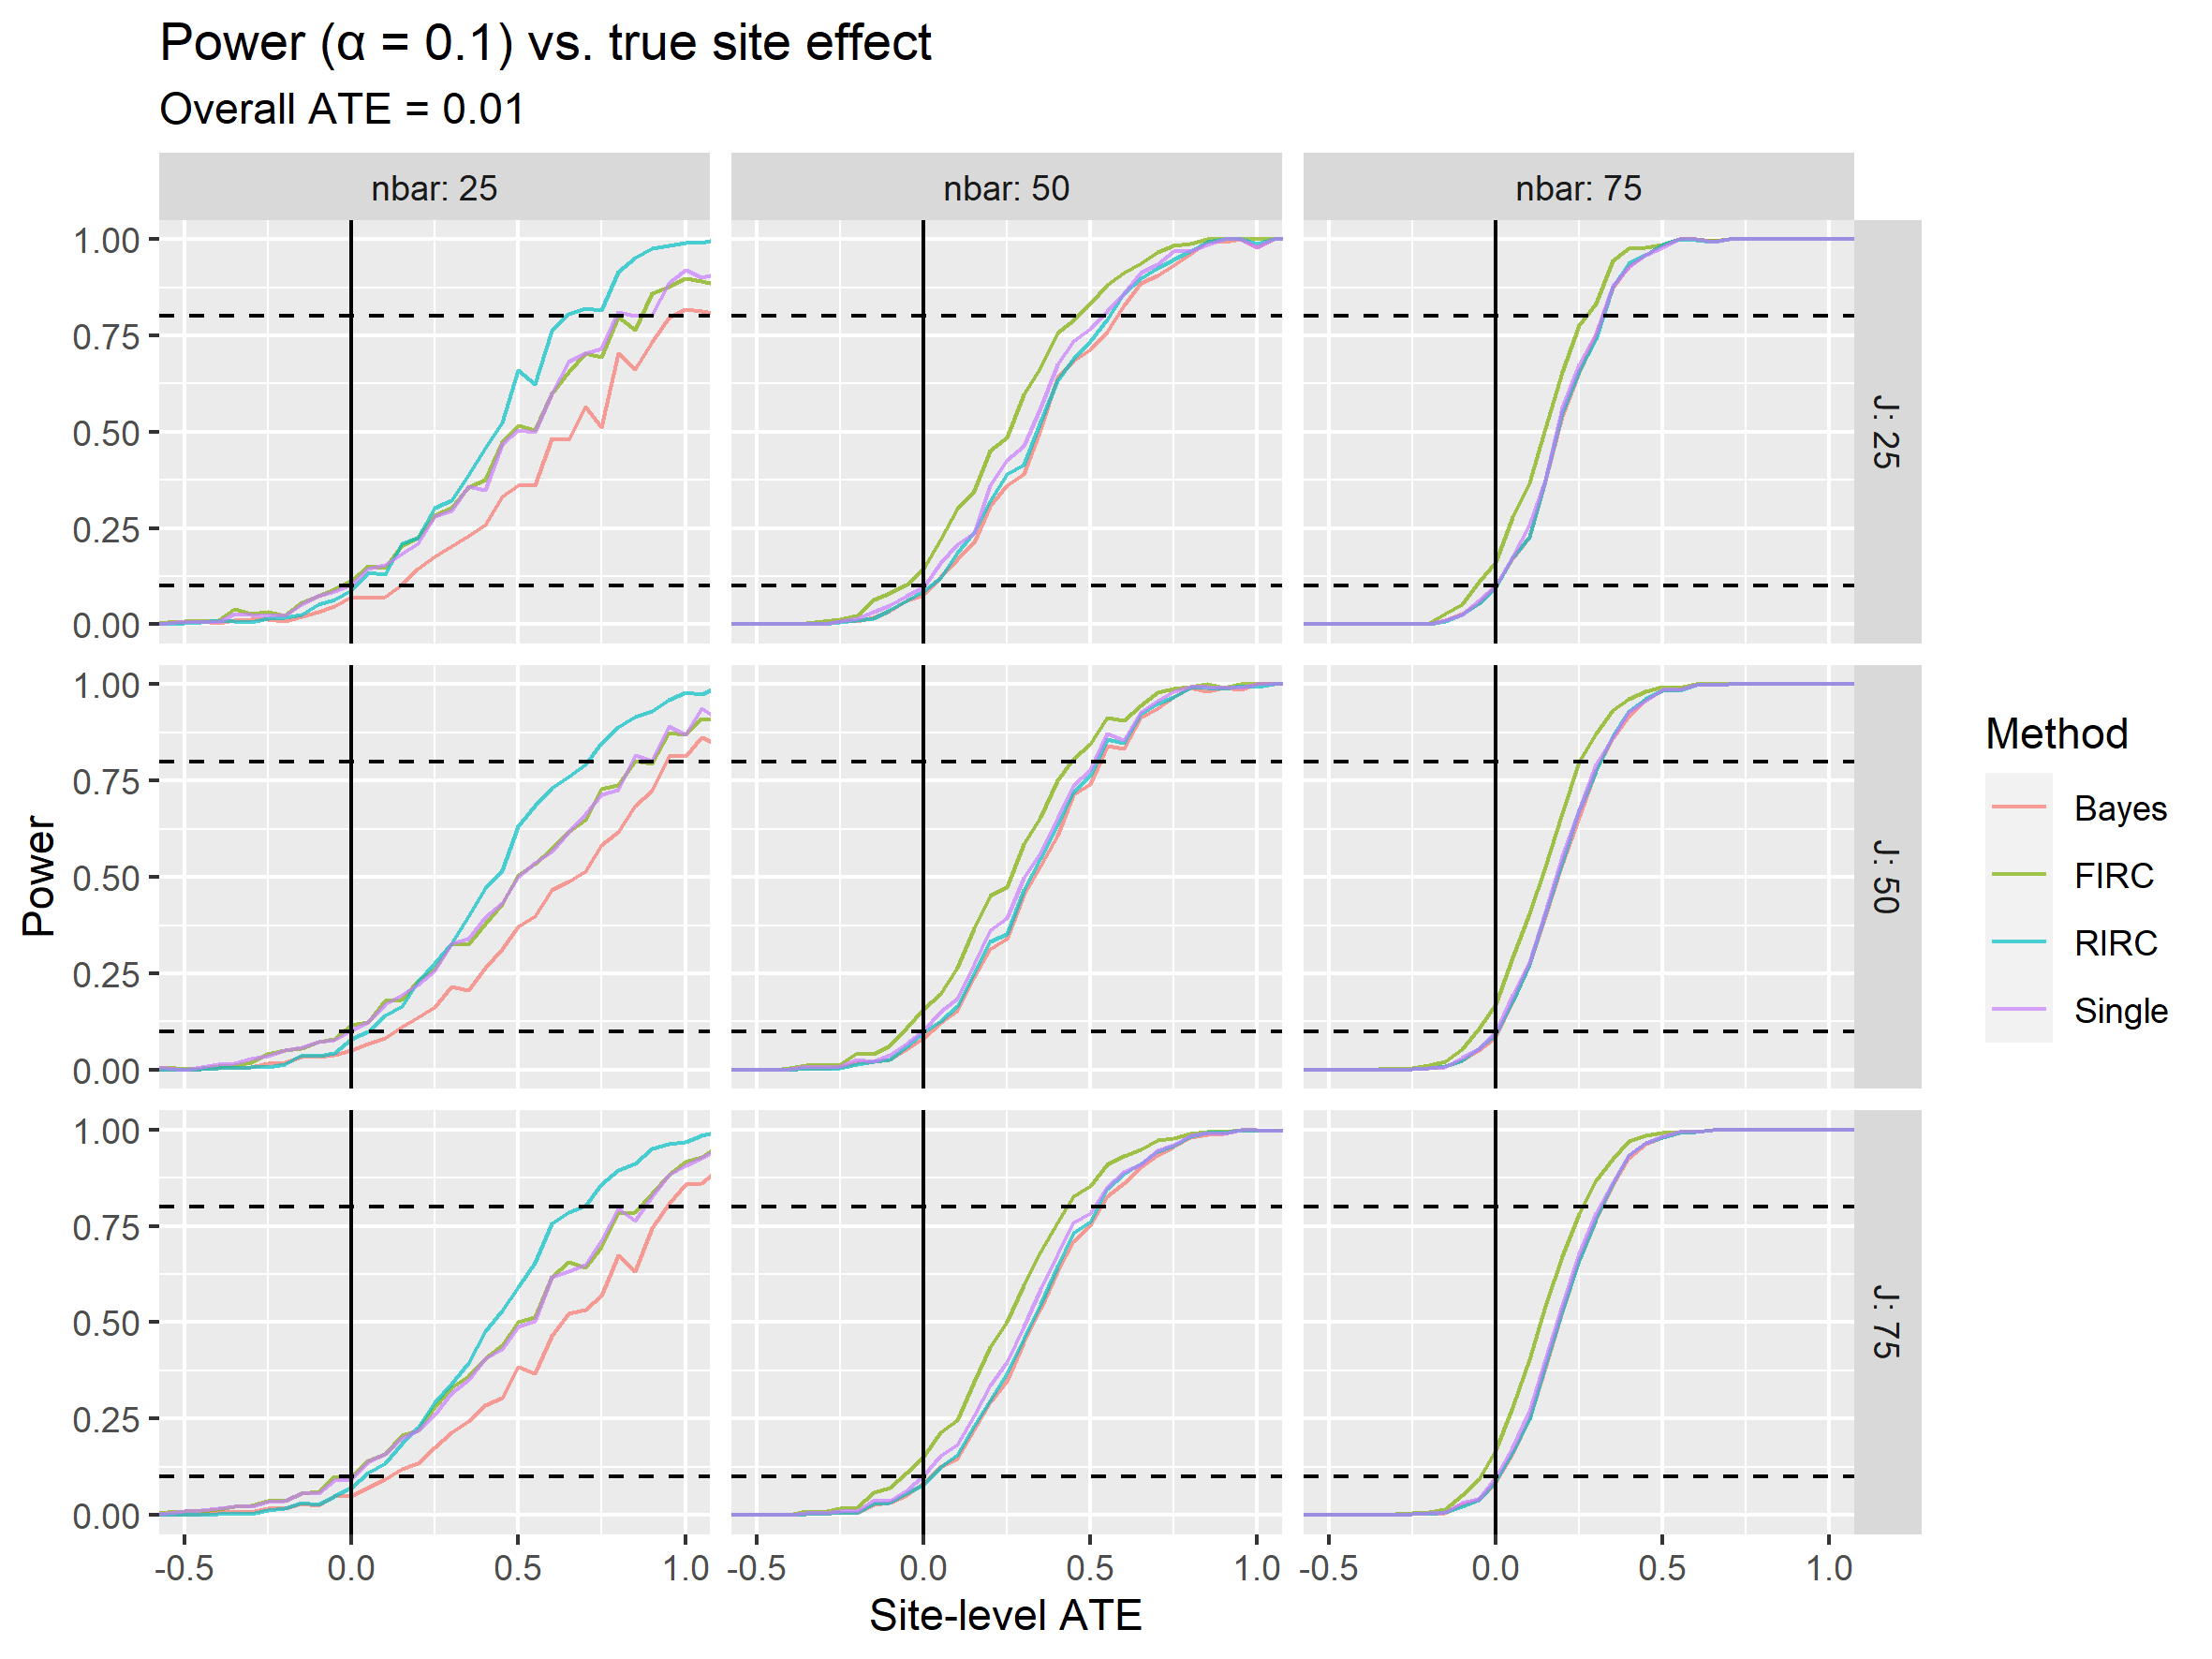
\includegraphics[width=\textwidth]{power_plot_01}
	\caption{Plot of power (at $\alpha = 0.1$) vs. true site ATE, for $\tau = 0.01$}
	\label{fig:power_plot01}
\end{figure}

\begin{figure}[ht]
	\centering
	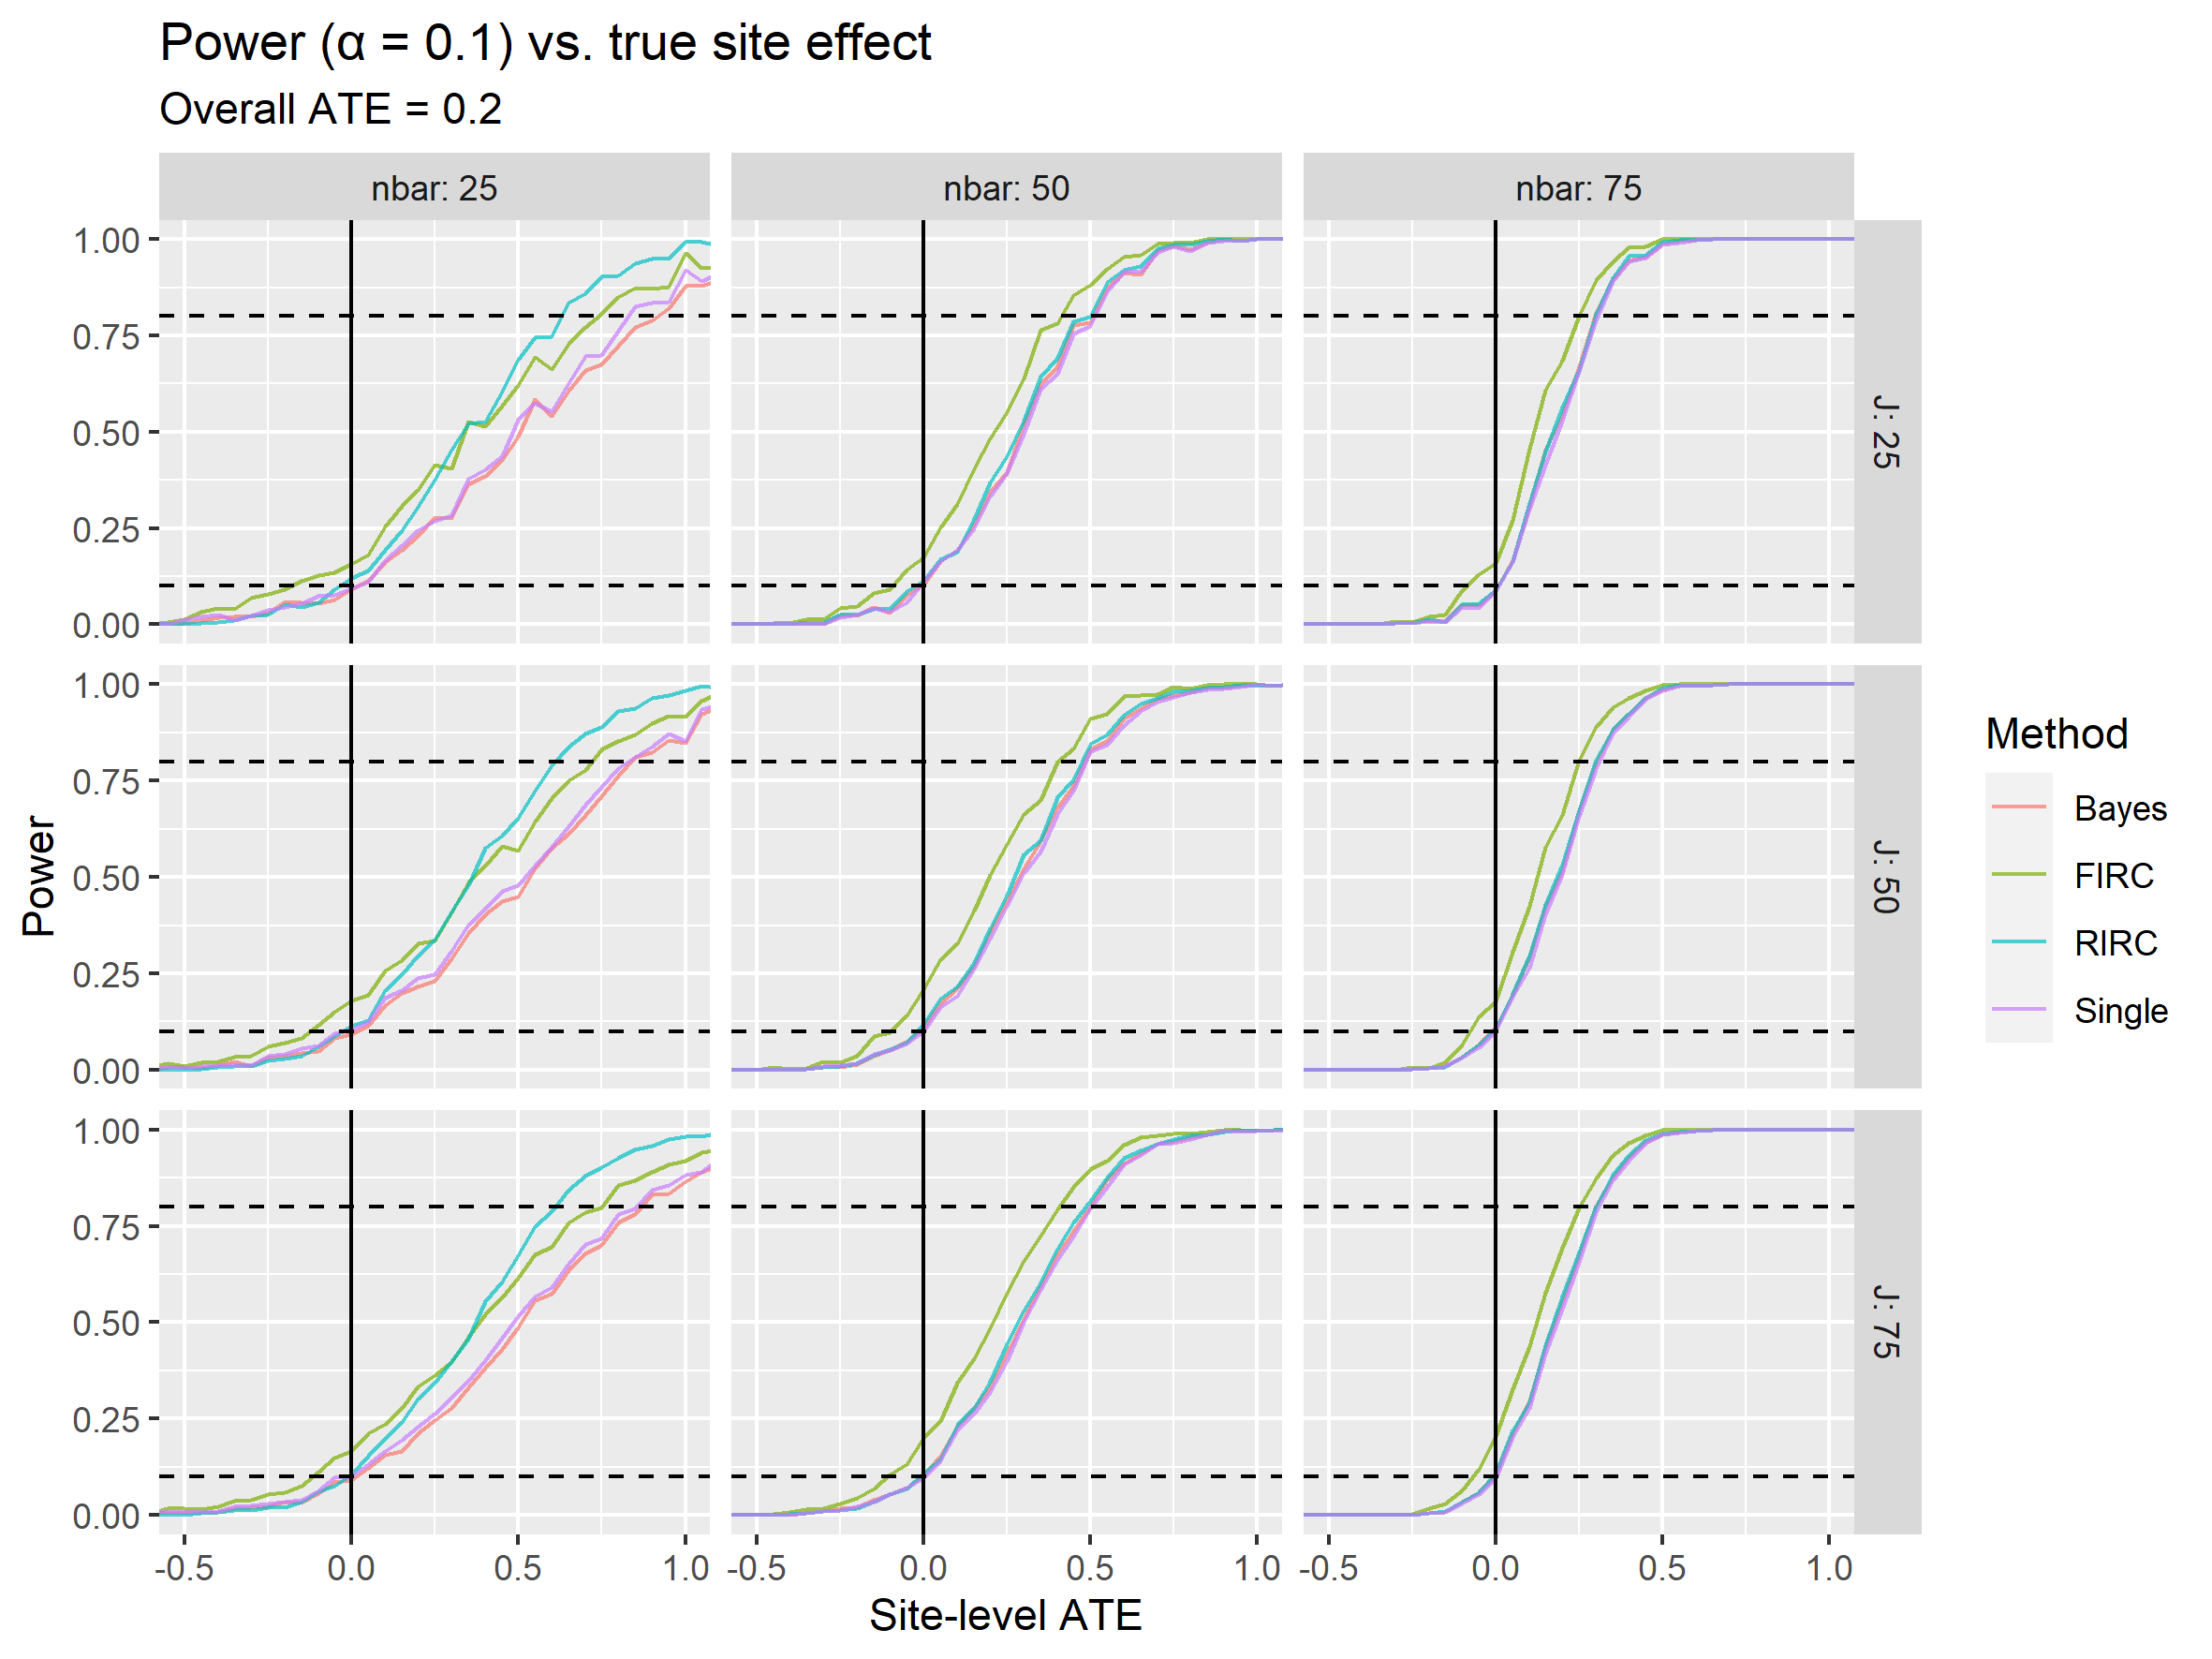
\includegraphics[width=\textwidth]{power_plot_2}
	\caption{Plot of power (at $\alpha = 0.1$) vs. true site ATE, for $\tau = 0.2$}
	\label{fig:power_plot2}
\end{figure}

\begin{figure}[ht]
	\centering
	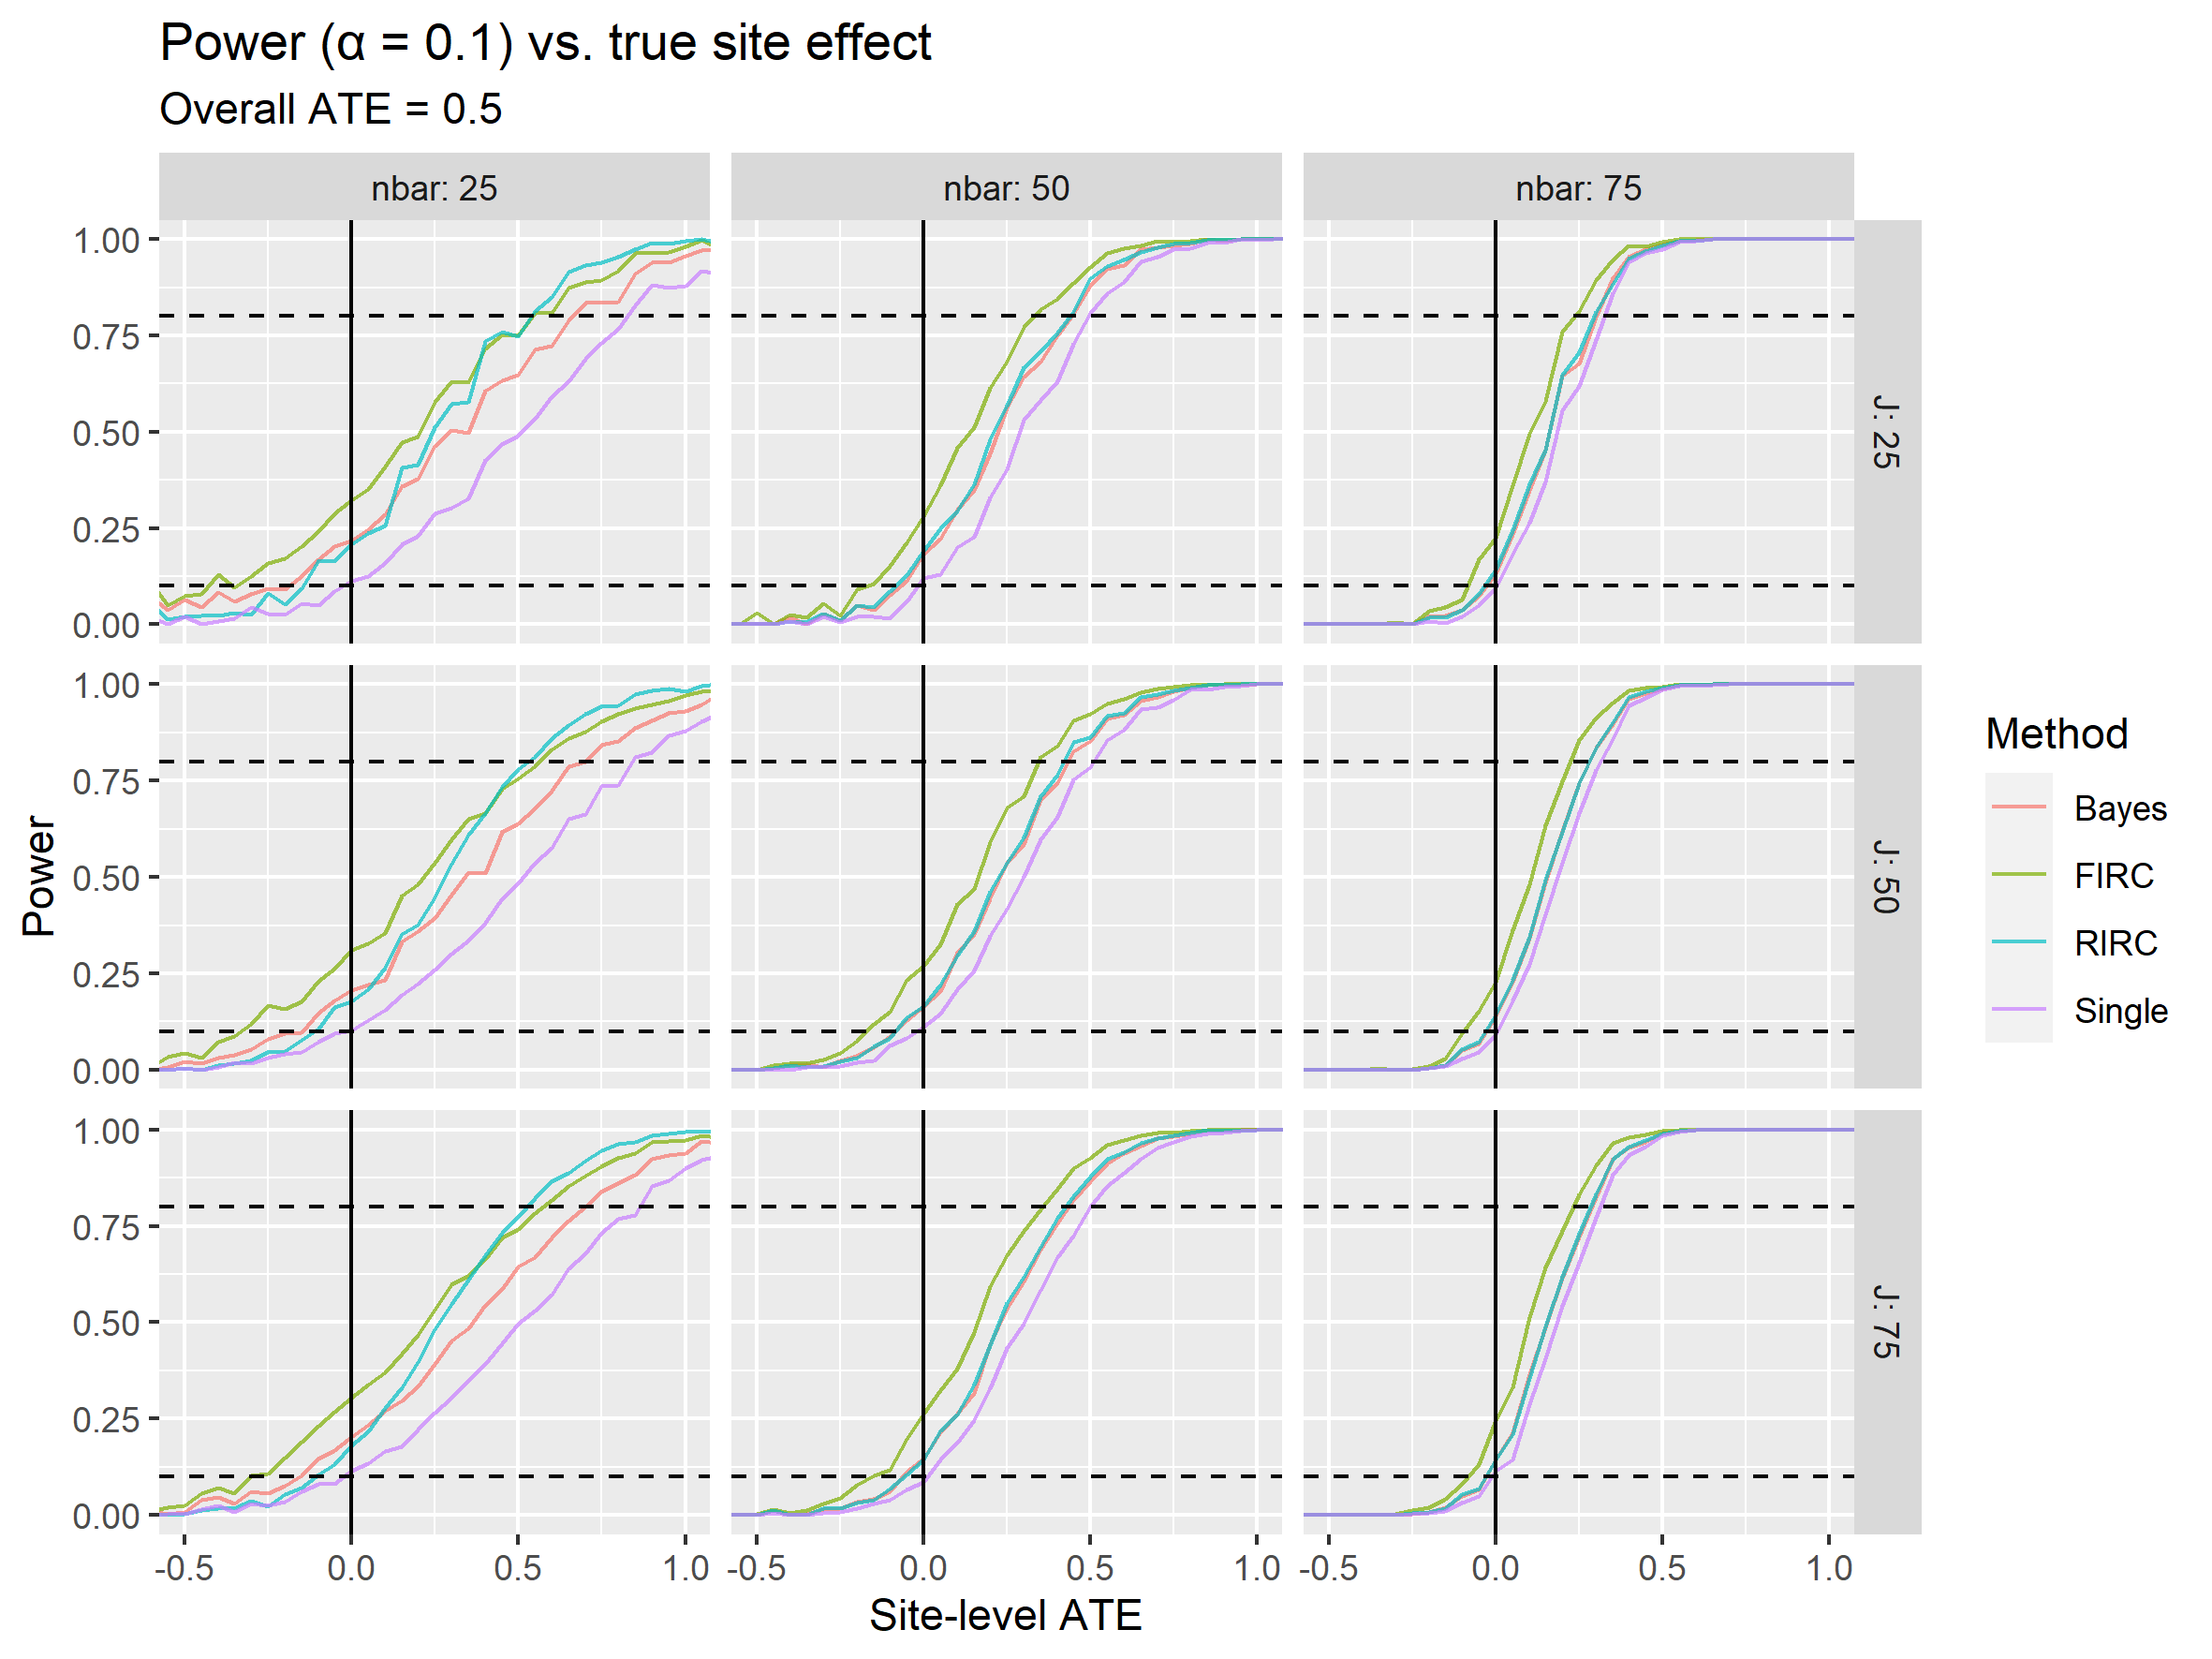
\includegraphics[width=\textwidth]{power_plot_5}
	\caption{Plot of power (at $\alpha = 0.1$) vs. true site ATE, for $\tau = 0.5$}
	\label{fig:power_plot5}
\end{figure}

Besides the three primary conclusions listed above, the power curves show a few interesting features.
First, we see that increasing $J$ does not affect the power for any particular $\tau_j$ (the curves remain the same from top to bottom).
While increasing $J$ naturally improves estimation of $\tau$, it does not significantly improve estimation of any $\tau_j$ values.
Second, we see that when $\bar{n}$ is small, we generally get bigger improvements in power for larger $\tau_j$ values.
This is related to our all-site simulation strategy; since sites are included in their own contexts, sites with large $\tau_j$ values increase the mean toward which they are shrunk, increasing power for those sites.
Finally, we see that the FIRC model has particularly bad false positive rates when $\tau$ is large.
(We are unsure about why this may be the case.)
Overall, none of the results are particularly surprising.
Using MLMs generally improves power, particularly when $\tau$ is high and estimates are shrunk upward away from zero.

We can also focus on sites for which $\tau_j = 0.2$ effect-size units, which is a reasonable moderate effect that we would like to be able to detect in a multisite trial.
Unfortunately, the power curves clearly show that it is difficult to achieve 80\% power when $\tau_j = 0.2$, with significant undercoverage in all but the most highly informative scenarios.
In general, MLMs are still only able to detect large effects ($\tau_j \approx 0.5$) with any sort of consistency.
We do, however, note that MLMS provide decent improvements in power in certain settings.
In the most extreme case ($\bar{n} = 25, \tau = 0.5$), we see that MLMS provide about a 30\% increase in power for sites with $\tau_j = 0.2$ relative to just using a single site, but this comes at the cost of a highly inflated false positive rate.
In a more standard setting ($\bar{n} = 25, \tau = 0.2$, we see about a 12\% increase in power, without a significant inflation of the false positive rate.
Once sites become informative enough, the power boost goes away.

To dig deeper into sites with $\tau_j = 0.2$, Figure \ref{fig:power_plot_ATE02_dens} plots density curves of estimated $\hat{\tau}_j$ values for each model when the true site effect $\tau_j = 0.2$.

\begin{figure}[ht]
	\centering
	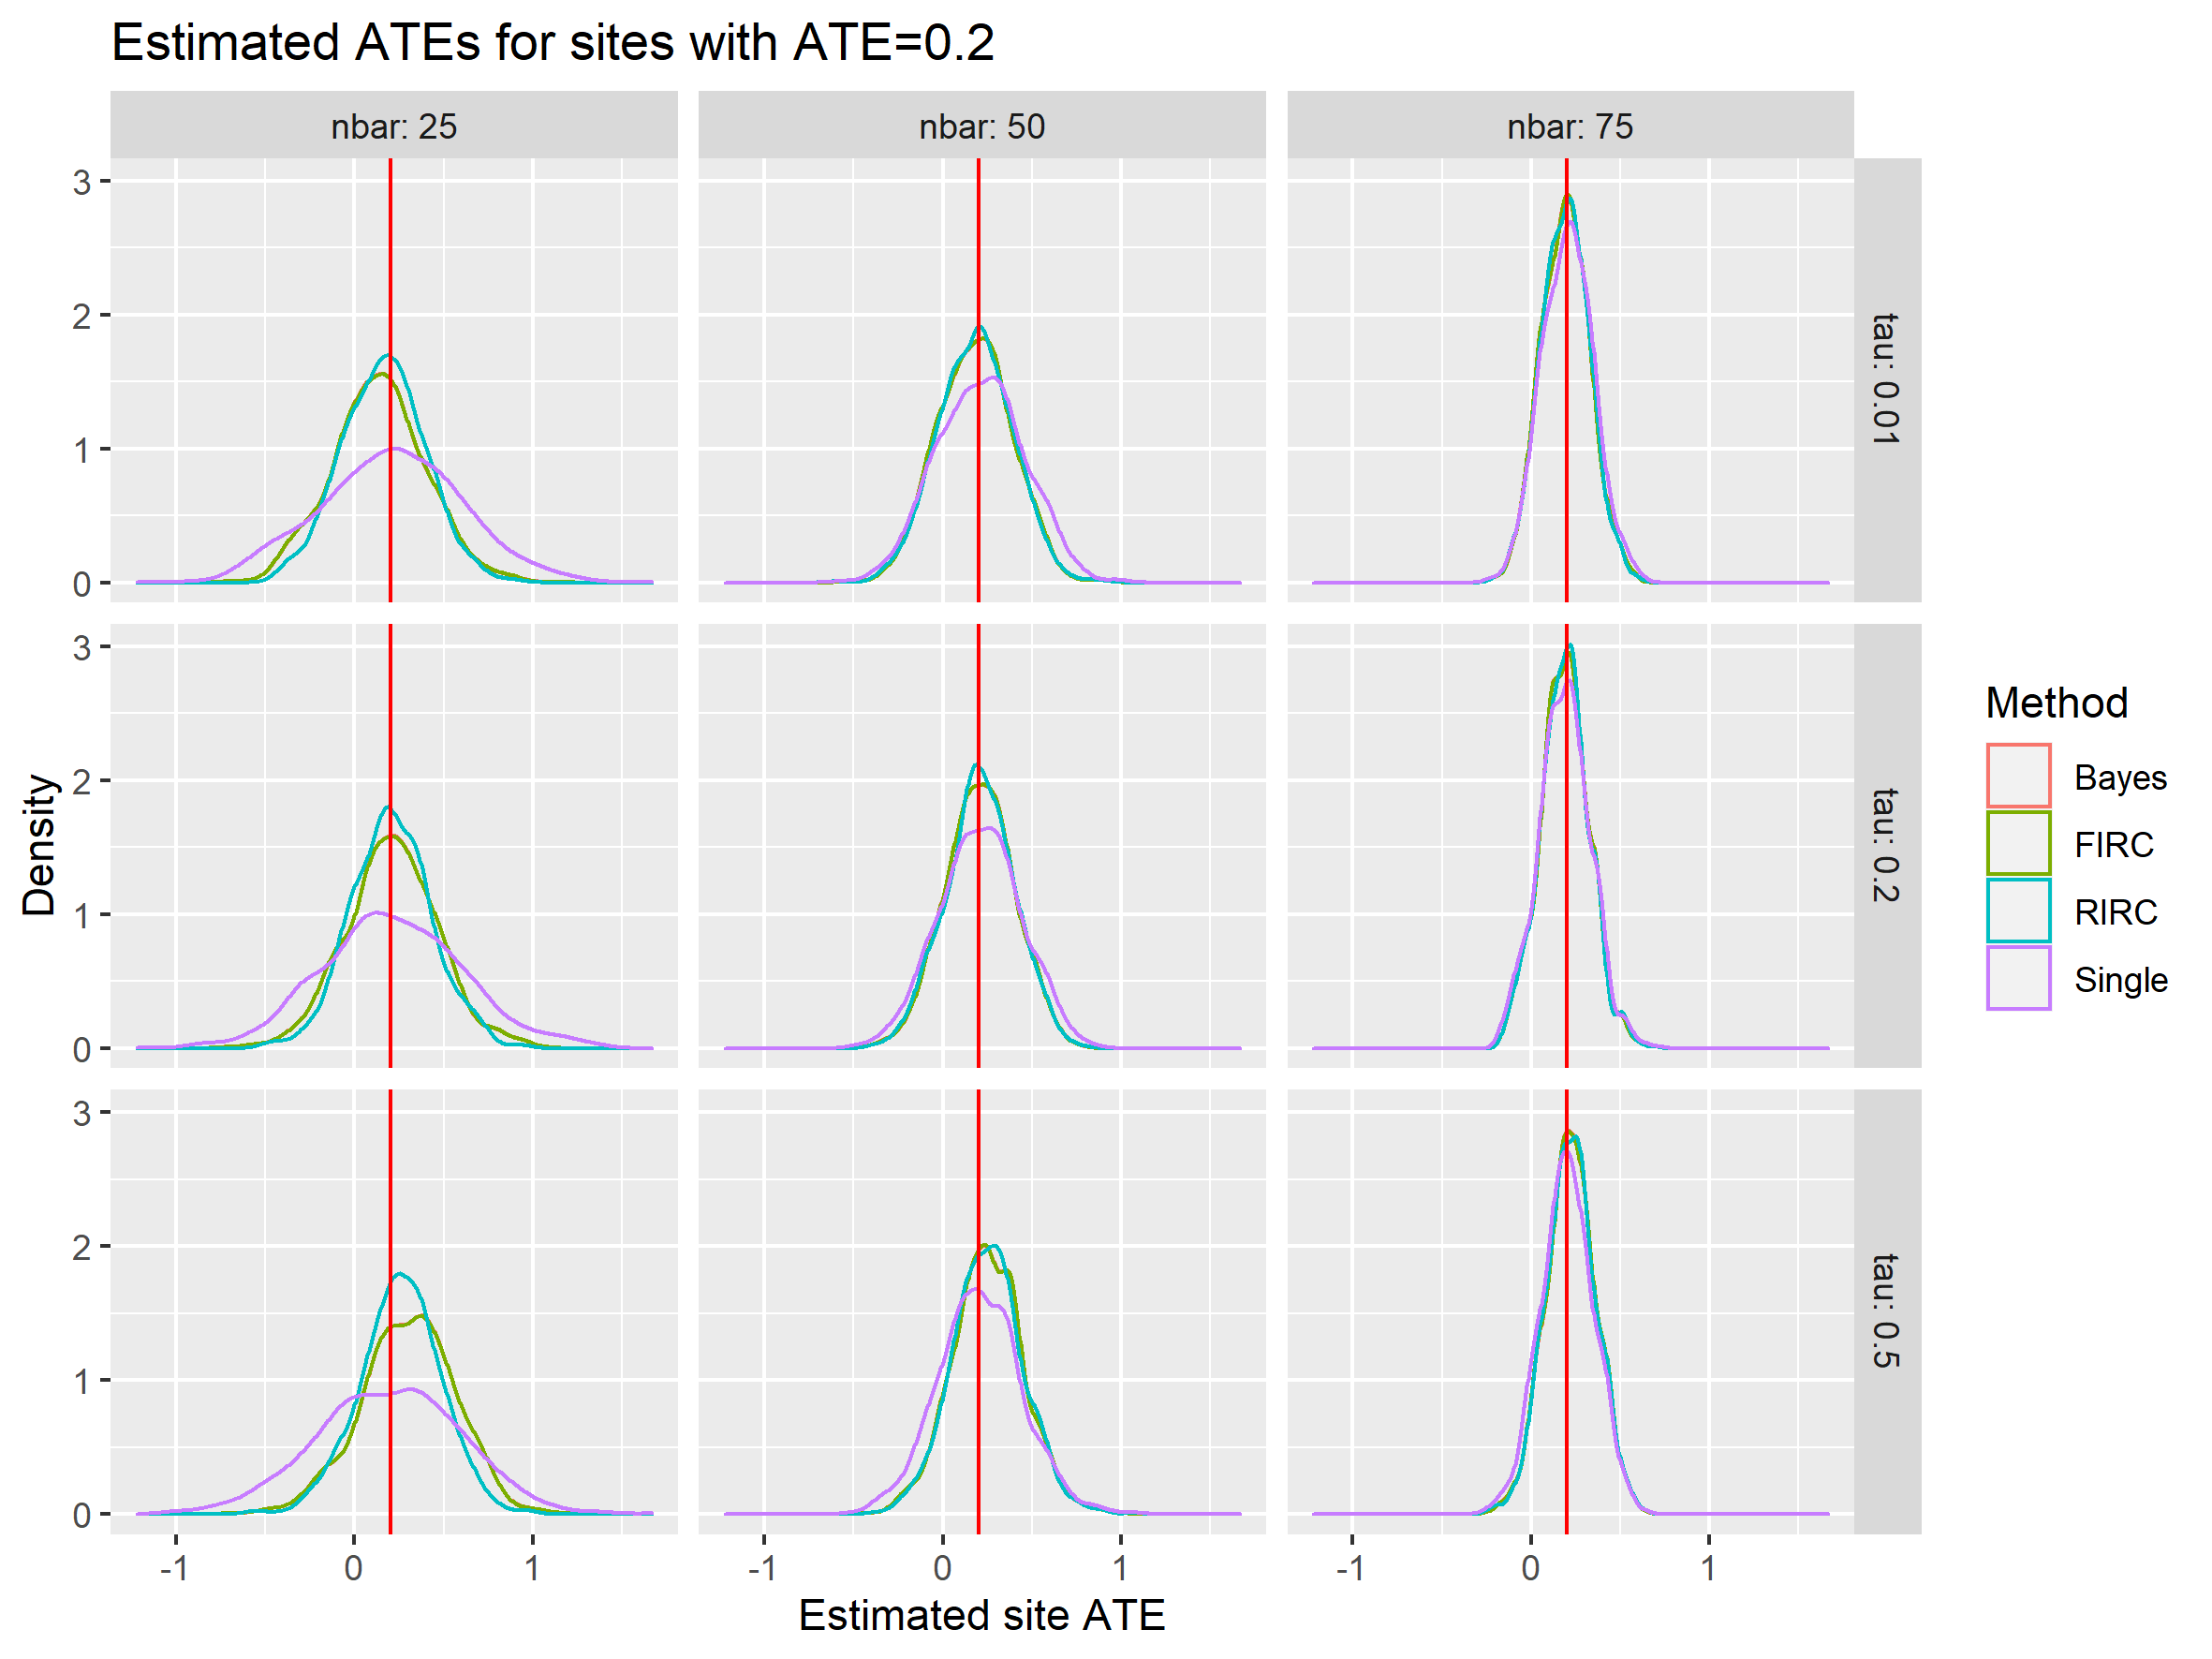
\includegraphics[width=\textwidth]{power_plot_ATE02_dens}
	\caption{Densities of estimated $\hat{\tau}_j$ values for $\tau_j = 0.2$ ($J = 50$)}
	\label{fig:power_plot_dens}
\end{figure}

We that as $\tau$ increases, estimates get shrunken toward greater values, so the density curves shift slightly toward the right.
The effect disappears as the sites become more informative.
In all cases, however, we clearly see that all methods produce many $\hat{\tau}_j$ estimates close to zero.

\subsection{Results: coverage}

We can also examine the coverage rates of the confidence intervals for $\tau_j$ computed under the different models.
Figure \ref{fig:coverage_plot} plots the coverage rate of 90\% confidence intervals against the true $\tau_j$ value.
Coverage rates don't change with $J$, so we only visualize results for $J = 50$.

\begin{figure}[ht]
	\centering
	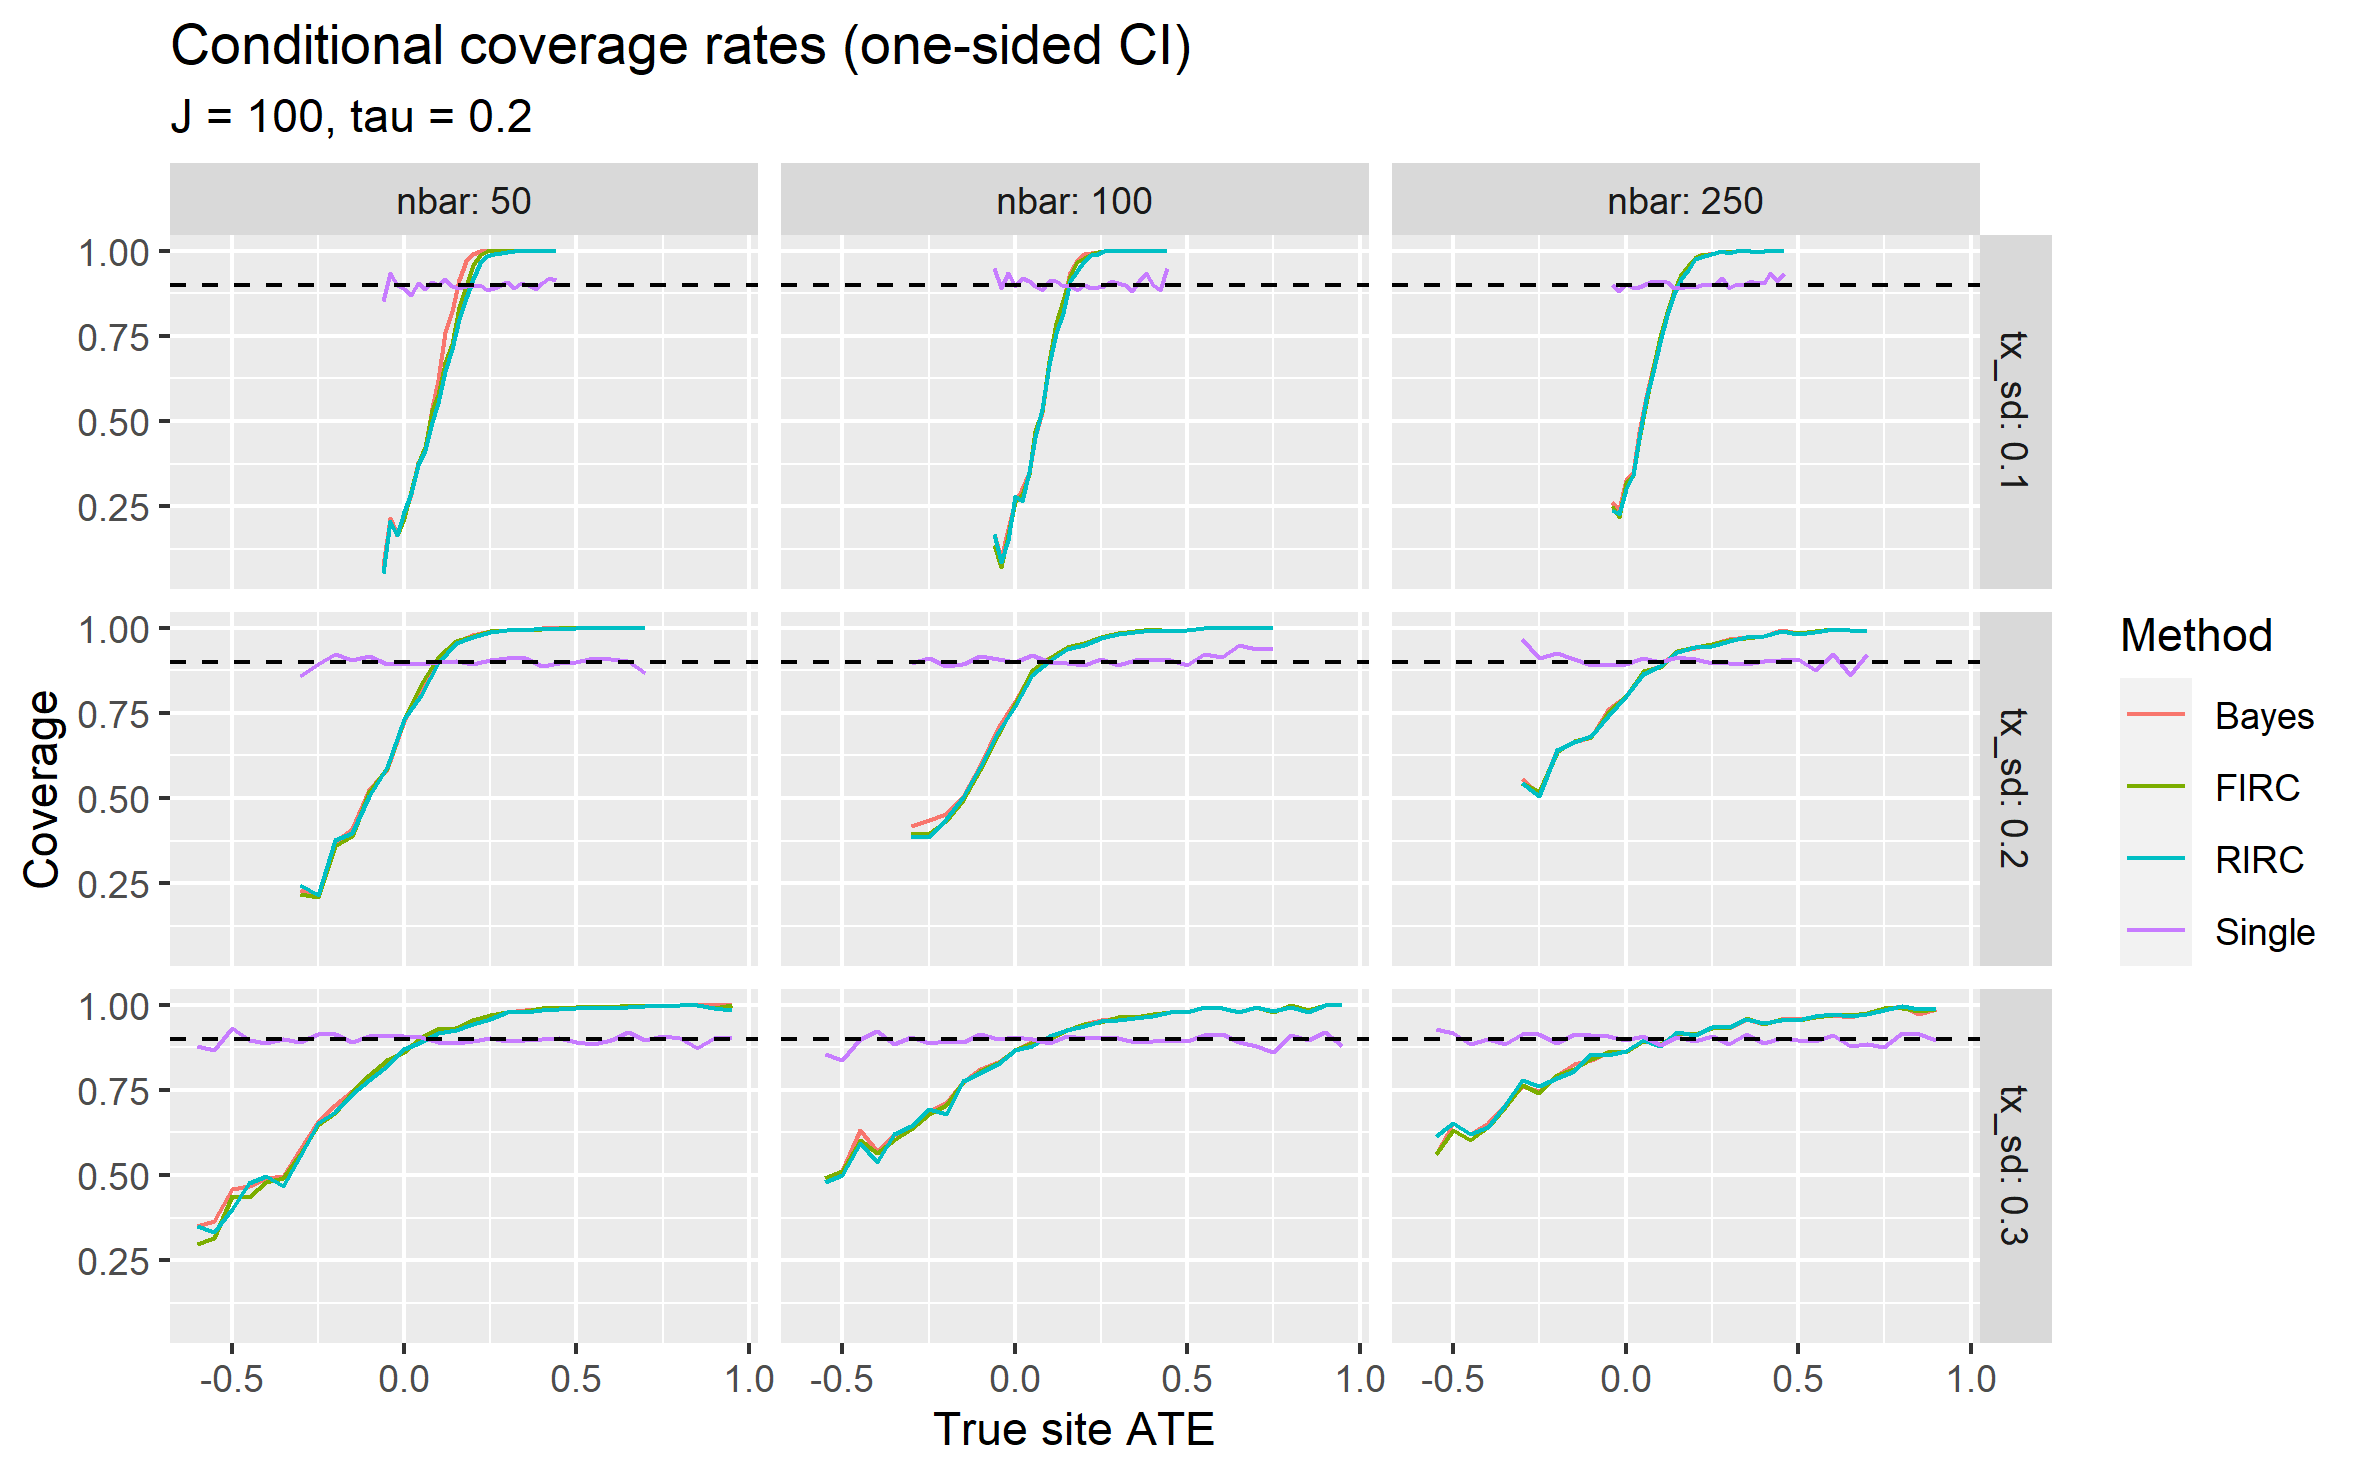
\includegraphics[width=\textwidth]{coverage_plot}
	\caption{Coverage of 90\% confidence intervals for each $\tau_j$ value}
	\label{fig:coverage_plot}
\end{figure}

While the single-site estimates obviously have roughly 90\% coverage regardless of the value of $\tau_j$, we see curvature in the coverage curves for MLMs; sites with $\tau_j$ values close to $\tau$ are overcovered, and sites with $\tau_j$ values far from $\tau$ are undercovered.
This sort of behavior is expected when examining Frequentist coverage of Bayesian procedures, where shrinkage induced by prior information or, in this case, a second-level model on the $\tau_j$ values, results in overcoverage for true parameter values near the center of shrinkage at the cost of undercoverage for parameter values far from the center of shrinkage.\footnote{Averaging this coverage over a distribution of $\tau_j$ values would give us EB coverage, which is approximately 90\% for all of the methods besides FIRC (plot not shown).}

We notice that the curvature in the coverage curve is the most extreme when sites are uninformative (and the model does a significant amount of shrinking), and that it becomes less extreme as the sites grow more informative.
We also see that while coverage for the single-site, RIRC, and fully Bayesian models appears to be approximately correct, the FIRC model seriously undercovers.
This undercoverage is not surprising, since for the FIRC and RIRC model we follow the standard practice of only using the standard error of the estimated random residual $\tau_j - \tau$, and not also adding in the standard error of the estimate of $\tau$.
It is somewhat more surprising that the RIRC model is approximately correct even without incorporating the standard error of the estimate of $\tau$.

\textit{Note to self: there's something weird going on with the simulated samples of $\tau_j$ (which we're not currently using).
For both FIRC and RIRC, the standard error of the random effects as computed via se.ranef doesn't match the empirical standard deviation of the random effects samples!
For RIRC, this empirical standard deviation is basically zero for some reason...}


\subsection{Results: RMSE}

As a sidebar, we can confirm that using MLMs improves the root-mean-squared error $\sqrt{\frac{1}{J} \sum_{j=1}^J (\hat{\tau}_j - \tau_j)^2}$ (RMSE) of the collection of site-effect estimates.
Figure \ref{fig:rmse_plot} shows the RMSEs of our estimators across our 500 simulation runs.

\begin{figure}[ht]
	\centering
	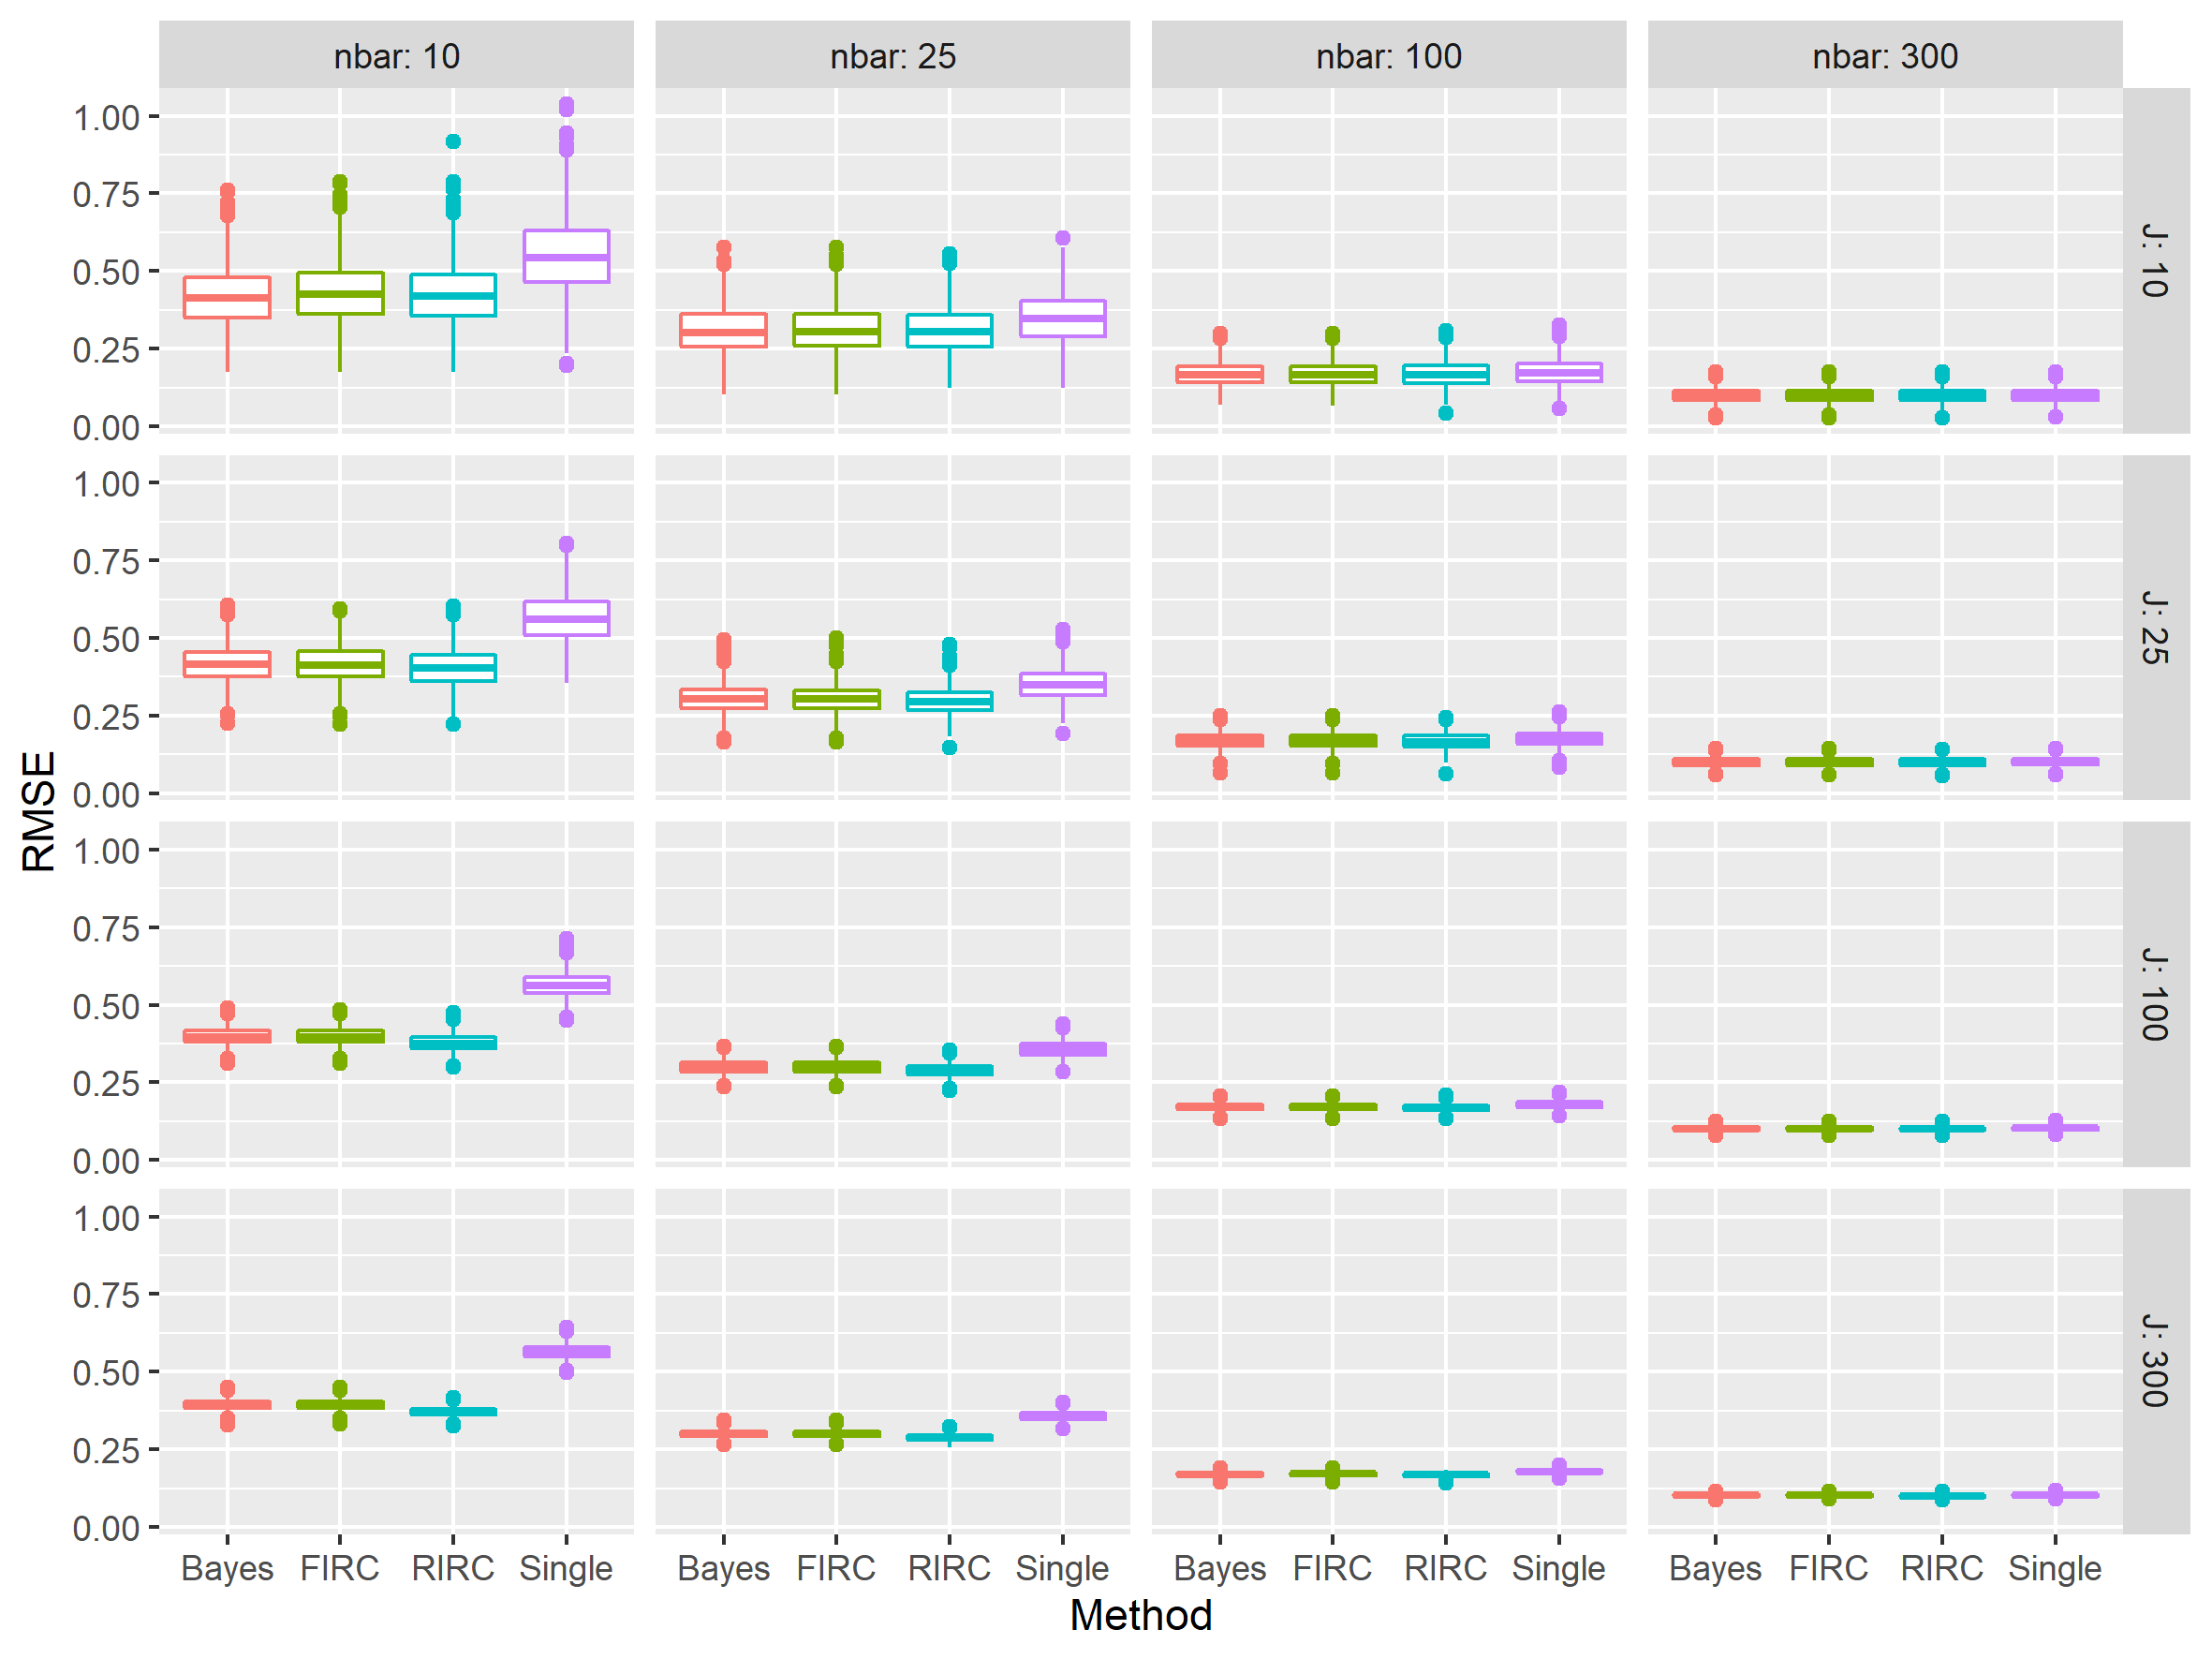
\includegraphics[width=\textwidth]{rmse_plot}
	\caption{Root-mean-squared error of site effect estimates}
	\label{fig:rmse_plot}
\end{figure}

We see that using MLMs indeed decreases RMSE as expected, with the decrease being largest for uninformative sites.
Interestingly, the RIRC model seems to perform particularly well in terms of RMSE.


\subsubsection{Discussion}
Overall, MLM shrinkage slightly increases rejection rates, relative to single-site estimates.
This effect is the most visible when sites are uninformative and the overall average effect $\tau$ is high.
The increase in power, however, is not particularly strong (<10\%) for sites with small to moderate (<0.5) effect sizes.
When comparing different MLMs, we saw that while the FIRC model rejects the null more frequently than the RIRC and fully Bayesian models, it does so at the cost of an inflated type-I error rate.
As such, we recommend the use of the RIRC or fully Bayesian models, which appear to have slightly greater power than single-site estimates, while maintaining approximate frequentist coverage properties.

%In most cases, power is low: MLM is not allowing for any reasonable level of rigor in investigating individual site effects.
%That being said, if one really does want a decent guess as to an individual impact, MLM is a far better option, in this context, than the simple difference.


\appendix
\section{Appendix A: model details}

TODO: describe details of Bayesian MLM

%TODOs:
%\begin{itemize}
%	\item Singular fit rate analysis
%	\item Show that rounding $\tau_j$ isn't a horrible sin
%\end{itemize}

	
\end{document}